%Chapter 1

\renewcommand{\thechapter}{1}

\chapter{Introduction}

\section{Extragalactic Astronomy: The beginning}
Nebulae, which stand for clouds in Latin, have been an integral part of astronomy since the Middle Ages and were one of the main driving forces behind extragalactic hypotheses. Their first known record dates back to 150 AD, who recorded five objects in the sky as ``nebulous'' in his books VII-VIII  of \textit{Almagest}. Abd al-Rahman al-Sufi noted a ``little cloud'' during 964 AD in his work \textit{Book of fixed Stars}, which we now know as the Andromeda Galaxy. On July 4th, 1054, Chinese and Persian astronomers have recorded the supernova event of the Crab nebula.

With the advent of refracting telescopes, mainly built based on the designs developed by Hans Lippershey in the early 17th century, Orion nebula has been detected and studied in detail by French and Swiss astronomers. Several more nebulae have been cataloged by the middle of the 18th century. In 1715, Edmund Halley published a list of six, Jean-Philippe de Cheseaux twenty with eight newer ones in 1745, Nicolas Louis de Lacaille 42 between 1751-1753. Later in 1781, Charles Messier compiled a list of 103, which are now called Messier objects, including the famous M87.

The number of known objects substantially improved with the works of William Herschel and his sister Caroline who published catalogs with more than a thousand nebulae during the 1780s. However, it was unclear at the time whether some of these objects were located outside the Milky Way. Based on the work of \cite{wright1750original}, who explained the Milky Way as a humungous spinning disk with several layers of stars, \cite{kant1797allgemeine} hypothesized that some nebulae with a fuzzy spiral shape might be independent Milky Ways themselves and termed them ``island universes''. He also suggested the others were thin gas and dust clouds within the Milky Way, collapsed into a spinning disk forming stars and planets, commonly called the nebular hypothesis--both commonly interpreting nebulae as collections of stars.  \cite{10.2307/106755} later noted a reddish region in the central regions of Andromeda, which did not appear anything like a star or known gaseous nebulae, advancing Kant's extragalactic hypothesis. These results resulted in an intense debate in the community. Many astronomers sided with Laplace, who maintained the nebular hypothesis view for spiral nebulae, while a few believed in the extragalactic origin. 

\citet{huggins1864xiii} noted that the spectra of Andromeda resemble a continuum overlaid with absorption lines and concluded that they were stellar in nature. \citet{fath1909spectra} found similar spectra in a few more nebulae. Interestingly some emission lines from one nebula, NGC 1068, were found to have a width of  $\sim$3000 km/s, similar to the lines found in nearby gaseous nebulae, supporting both the hypotheses. Later \citet{slipher1913radial} noted that the lines from Andromeda display a redshift higher than the escape speed of Milky Way, thereby indicating an extragalactic origin. These conflicting views sparked the ``Great Debate'' in astronomy \citep{1921BuNRC...2..171S} between Harlow Shapley and Heber Curtis in April 1920, each favoring the nebular and extragalactic views, respectively, based on different arguments. For example, Shapley argued that the energy output of the nova observed in Andromeda \citep{1888MNRAS..48..108B} would be physically impossible to explain if it were an external galaxy. Conversely, Curtis showed that the nova events in Andromeda outnumbered those in Milky Way and questioned why the events must be disproportionately large in a specific region of the Milky Way if Andromeda were to be a part of it.

Later, \citet{opik1922estimate}  estimated the distance of Andromeda to be about 450 kpc (which is half the actual value), placing it well outside our Galaxy. The debate was finally settled in the late 1920s by \citet{hubble1929relation} who used Cephid variables to confirm Andromeda's extragalactic origin. Cephids are stars with a cycle of brightness whose frequency correlates with their luminosity, allowing us to determine their distance. 

\section{Active Galactic Nuclei: A new paradigm}
Although Hubble's work validated the presence of extragalactic objects, the nature of the bright emission lines from centers some galaxies, however,  remained unknown for a decade or two.  \citet{seyfert1943nuclear} obtained the spectra of six galaxies and found that they show high-excitation emission lines superimposed on a solar-like continuum with widths reaching up to 8500 km/s. These types of galaxies are now called as \textit{Seyfert Galaxies}.  \citet{woltjer1960magnetostatic} noted that parsec scale emission from these galaxies requires a mass of $\sim 10^8$ solar masses ($M_\odot$). \citet{fowler1963star} made an important advance by suggesting that the centers of these galaxies host a massive star; they would emit by accreting dust from the surroundings. A year later, another idea emerged, which assumed that the central object is a black hole rather than a massive star \citep{salpeter1964accretion,zel1964estimating}. Such galaxies, whose bright centers are powered by accretion onto a black hole, are what we now call Active Galactic Nuclei (AGN). AGN are the most luminous and steady sources of luminosity in the universe. They have a broad spectrum covering 20 orders of magnitude in frequency, and their luminosity ranges from $10^{40}-10^{49}$ ergs s$^{-1}$ and are one of the most actively studied classes of objects in astronomy.

\subsection{Radio Astronomy}
Radio astronomy also provided essential contributions to our understanding of AGN. Its history dates back to the early 1930s. In 1932, Karl Guthe Jansky, an engineer at Bell Labs, noted that a radio signal peaked with a period of 24hrs and suspected that they were radio waves from the Sun. Upon gathering more data, he found that the signal repeated with the frequency of a Sidereal day: the time it takes for distant stars to rotate once in our field of view. These findings eventually led Jansky to conclude that the signal came from the central regions of our galaxy \citep{jansky1932directional}, and it marked the first serendipitous discovery of an astronomical radio source and the birth of radio astronomy. He was honored for his seminal contributions to this field by naming the units of flux as Jansky (Jy) after his name.

Inspired by this discovery, Grote Reber, an amateur radio engineer, built a parabolic radio telescope in his backyard with a 9m diameter. He mapped the emission from the galactic center at 160 MHz and not only confirmed Jansky's discovery \citep{reber1940cosmic} but also showed that the emission exhibits a non-thermal spectrum. Although World War II intervened during this period and hindered research in astronomy, it led to advances in radar technology and, consequently, in radio astronomy. 

Martin Ryle and Antony Hewish developed Earth-rotation aperture synthesis techniques in the 1950s, allowing emulation of a large aperture-telescope using a network of several spatially-separated smaller telescopes called baselines. With the arrival of efficient computing machines capable of performing the required inverse Fourier transforms, it was possible to build radio telescopes with one mile and later with 5 km apertures. These telescopes 
%The brightness temperatures of some sources are greater than $10^6 K$ and indicate a non-thermal origin \citep[e.g.,][]{bolton1948variable}. 
%\citet{1950AuSRA...3..234S} located a bright radio source that coincided with the location of M87, which we now identify as a nearby AGN. Later, \citet{1954ApJ...119..215B} identified extended optical emission from M87.
were used to conduct the 3C and 3CR sky-surveys at 159 MHz and 178 MHz, respectively, detecting several hundreds of radio sources \citep{1959MmRAS..68...37E,10.1093/mnras/125.1.75} including well-known sources like 3C 48 and 3C 273. While some had extremely faint star-like optical detections showing emission lines matching with no known element on earth at that time \citep{1963ApJ...138...30M}, the low resolution of these surveys precluded accurate identification of optical counterparts for many of them. Their optical variability ruled out a normal galaxy-like origin, and their extreme brightnesses prevented a stellar interpretation, leading astronomers to call such sources as \textit{quasi-stellar (star-like) sources}, shortened to \textit{quasar} \citep{chiu1964gravitational}. 

\subsection{Discovery of Quasars}
A few years later, measurements of 3C 273 based on lunar-occultation technique allowed  \citet{schmidt19633c} to identify its optical counterpart with a magnitude of 13, again showing unknown lines; it also contained a structure he referred to as ``a faint wisp or jet.'' They both lay close to the radio positions of two bright components in 3C 273. The optical spectrum of  3C 273 exhibited a complex continuum with broad emission lines \citep{oke1963absolute}.
\citet{schmidt19633c} showed that the emission lines from 3C 273 match Balmer and Mg II lines at a redshift of $z=0.158$. Furthermore, \citep{oke1963absolute} found that a previously unidentified line in the infrared matched with an H$\alpha$ line with this redshift. A similar interpretation led to determining the redshift of 3C 48 as 0.37. These redshifts implied an extragalactic origin and a higher than typical luminosity.

After \citet{salpeter1964accretion} and \citet{zel1964estimating} advanced the idea of a black hole at the center of an AGN, \citet{lynden1969galactic} put forward an idea that accretion onto black holes with sufficient mass can power the high luminosity of quasars. He also argued that it could produce the observed thermal continuum and broad emission lines and be the process behind quasars and Seyfert galaxies. The community rapidly accepted this idea, marking the dawn of the basic AGN paradigm. Astronomers now widely believe that practically all the galaxies host a supermassive black hole (SMBH) at their center \citep[e.g.,][]{richstone1998supermassive}, and power AGN via accretion. The Event Horizon Telescope provided direct evidence for the existence of an SMBH by imaging its silhouette in M87 \citep{2019ApJ...875L...1E}.

\subsection{Discovery of Relativistic Jets from AGN}
In the late 1960s, \citet{hogg1969synthesis} detected extended radio emission from M87, which was previously identified as a ``curious straight ray'' by \citet{curtis1918descriptions}, coinciding with its extended optical component. Soon high-resolution sky-surveys conducted by radio interferometers at Cambridge revealed extended emission from several new extended sources \citep[e.g.,][]{1973MNRAS.165..369N,turland19753c} with the majority showing two-sided jets while one-sided from quasars. Moreover, these structures spanned a wide range of radio powers. However, it remained uncertain what determined their presence or absence and the sidedness. It was with the commissioning of the Very Large Array (VLA) with unprecedented sensitivity and angular resolution several \textit{jets} could be delineated from diffuse radio structures \citep[e.g.,][]{bridle1984extragalactic}. In the mid-1960s, discoveries of optical variability and detection of several unresolved radio sources with growing baselines indicated the presence of small-scale structures in some radio sources. These discoveries triggered the development of Very Long Baseline Interferometry (VLBI), a technique capable of detecting structures much smaller than the VLA, leading to the first detection of an apparent superluminal (or faster than light) motion \citep{whitney1971quasars,cohen1971small}, implying relativistic speeds. Several similar detections followed, and it began to be established that the observed extended morphologies are manifestations of relativistic radio jets from AGN \citep{blandford1979relativistic,konigl1980relativistic}, which from the broad subjects of my thesis. As an example, I show a VLA 8.4 GHz radio image of the one-sided jet in M87 in Fig.~\ref{fig:M87_showpiece} at 0.2\as~resolution. Despite the actual presence of twin jets in this source, due to a phenomenon called \textit{Doppler Boosting}, which I discuss in section \ref{subsec:relativistic_effects}, the emission from the approaching jet is amplified while is diminished for the receding jet, making it undetectable.
\begin{figure*}
    \centering
    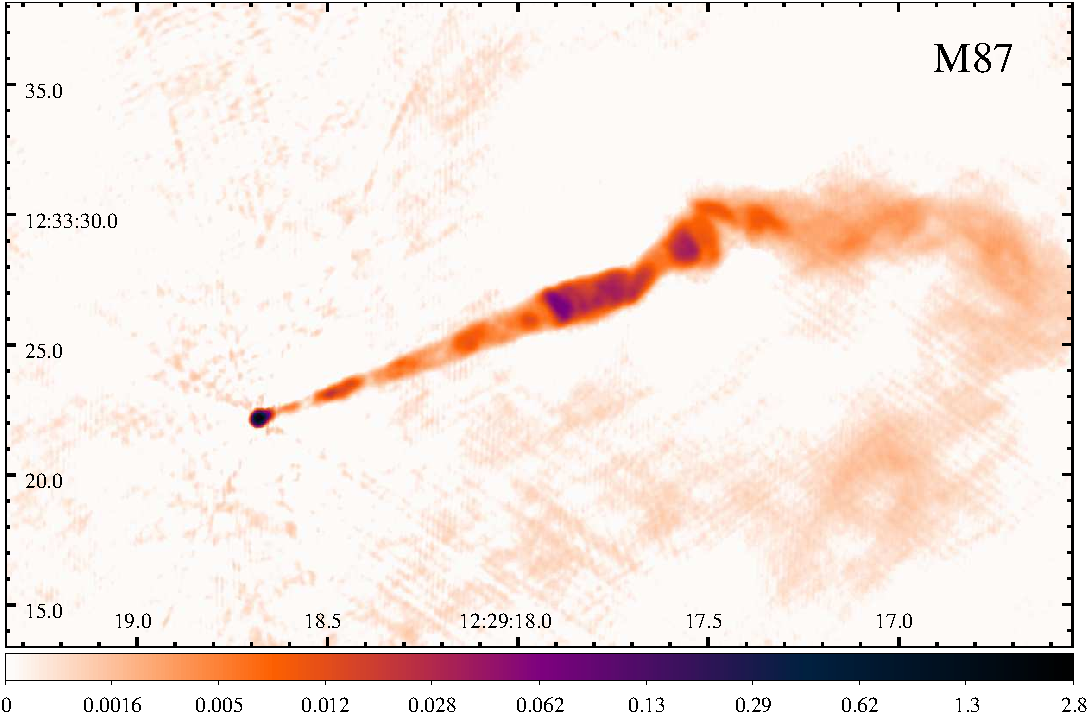
\includegraphics[width=0.849\textwidth]{images/misc/M87_thesis_showpeice-crop.pdf}
    \caption{A VLA 8.4GHz radio image of the relativistic jet in M87 \label{fig:M87_showpiece}}
\end{figure*}

%\subsection{Importance of Jets}
While a few millions of AGN are detected so far \citep[e.g.,][]{Assef_2018}, only a small fraction of them produce radio jets \citep[e.g.,][]{ivezic2002optical,Padovani_2017}. They transport energy and momentum from the central sub-parsec scale regions of the AGN out to parsec scales and often to kilo-parsec (kpc) and Mpc scales, with the largest known jet reaching a size of 5 Mpc \citep{2022arXiv220205427O}, which is roughly 1/3rd of the distance between M87 and the Earth. Such jetted AGN are generally classified as `radio-loud' AGN. Although the exact jet launching mechanism is unknown, it is commonly believed that a strong magnetization of the accretion disk coupled with the black hole's spin produces outflows at relativistic speeds \citep[][]{blandford2019relativistic}.

The kinetic and radiative power output from these jets can stimulate and limit the growth of galaxies. It can also be responsible for producing high energy cosmic rays and intergalactic magnetic fields \citep[for a recent review, see][]{blandford2019relativistic}. It is plausible that the jets may have regulated black hole masses of the early universe \citep{churazov2005supermassive} via feedback. There is also growing evidence that jets may have shaped the baryonic (i.e., protons, neutrons, and alike) part of the local universe  \citep[][]{fabian2012observational}. If so, the jets have profound implications for the universe's evolution.

Despite the significant role that jets may have played in galaxy evolution, we only know a little about jet physics even after studying them for more than half a century. For example, 
their particle composition--electrons and positrons or electrons and protons---is uncertain, as is the speed of the jets on kpc to Mpc scales. It is also unclear how jets remain collimated across large distances. Importantly, for the present work,  how powerful jets emit X-rays hundreds of kpc away from the central AGN is unclear. Two of the main competing models, which I describe in the final section of this chapter, imply orders of magnitude differences in the total power that jets feed into their host galaxies and clusters. My thesis attempts to elucidate the properties of X-ray emission from such large-scale jets.

In the following section, I introduce the radiative processes appropriate for the study of jets and then discuss the current model of AGN. I then discuss its resulting taxonomy and models proposed to explain the observed properties of jets. I then provide a detailed description of the current state of X-ray emission from large-scale jets, the main subject of my thesis.

\section{Radiative processes \label{sec:radative_processes}}
The emission from large scale jets spans a wide spectrum ranging from radio to X-rays \citep[e.g., ][]{harris2002x,worrall2009x} and sometimes up to $\gamma$-rays \citep[e.g.,][]{Meyer_2019,2020Natur.582..356H}. The synchrotron mechanism has been successful in explaining the observed radio-to-optical spectra of all the jets and X-ray emission for most low-power jets \citep[e.g.,][]{2001MNRAS.326.1499H,marshall2002}. Inverse Compton (IC) scattering is another form of raditation that is regularly invoked in the context of large scale jets. Although several other mechanisms have been proposed, for example, magnetic reconnection, their applicability for X-ray emission for large scale is still unclear. Hence, I restrict my discussion to synchrotron and IC mechanisms in the following sections.
%This section provides an overview of the two main radiation processes and the involved relativistic effects.


\subsection{Synchrotron Radiation}
One of the most important characteristics of synchrotron radiation is a high degree (upto $\sim$70\%) of polarization.  This characteristic led to the first-ever proof that synchrotron radiation produces optical emission from the jet of M87 \citep{baade1956polarization}, and also quickly explained the radio emission from other jets.

 Charged particles, when accelerated, emit electromagnetic radiation  \cite[for a review, see][]{longair_2011}. If the charged particles are relativistic and are accelerated by a magnetic field, they produce synchrotron radiation.  The  power radiated by a charged particle (mass=$m$ and charge$=Z$) moving with a speed $v$ in a magnetic field $B$, is proportional to 
%energy $E=\gamma mc^2$ (where $\gamma$ is the Lorentz factor) and speed v 
\begin{equation}
      P_{synch} \propto \frac{Z^4\gamma^2B^2v^2 \sin^2\theta}{m^2}
\end{equation}
 where $\gamma$ is the Lorentz factor and $\theta$~is the pitch angle.  Because $P_{synch}\propto m^{-2}$, the emission is extremely efficient for electrons and positrons when compared to protons that are \siml 2000 times heavier. For an electron and proton travelling with the same speed, the power radiated by a proton will be smaller by a factor of $3\times10^{-7}$ compared to an electron. That means, for a given synchrotron luminosity, a jet with radiating protons would demand a significantly higher energy budget than an electron-jet. Because of this radiative efficiency, only electrons (or positrons) are generally assumed to be emitting in jets for the purpose of radiative calculations.
 
The average power radiated by an electron for an isotropic distribution of pitch angles is given by 
\begin{equation}\label{eq:synch_pow}
    \langle  P_{synch} \rangle=\frac{4}{3}\sigma_T\beta^2\gamma^2cU_B
\end{equation}
where $\sigma_T$ is the Thomson scattering cross-section, $c$ is the speed of light, $\beta=v/c$ and $U_B=B^2/8\pi$ is the magnetic field energy density, and $\gamma=1/\sqrt{1-\beta^2}$~is the Lorentz factor. Furthermore, 
the specific luminosity of a single electron spectrum peaks at $0.29\nu_{crit}$, where $\nu_{crit}$ is the critical frequency given by:
%An electron emits approximately half of the total power [WITHIN WHAT BAND PASS? MAYBE YOU WANT TO SAY THAT THE SPECIFIC LUMINOSITY EMITTED PEAKS AT 0.29 NUCRIT] at a \textit{critical frequency}, which is given by:
\begin{equation}
    \nu_c = \frac{3\gamma^2eB}{4\pi m_e c}\sin{\theta}
\end{equation}
where $e$ is the electron charge. That means, to produce synchrotron radiation at $\nu\sim1$ GHz in a magnetic field of $B\sim10^{-6}$ G, an electron  requires $\gamma\sim10^{4}$. Such extremely relativistic electrons in a jet can only be produced by an efficient particle acceleration mechanism, such as the first-order Fermi acceleration \citep{1949PhRv...75.1169F}.

The radio spectrum of a jet usually takes a powerlaw form $F_\nu\propto \nu^{-\alpha}$ where $F_\nu$ is the flux density,  $\nu$ is the frequency, and $\alpha$ is the spectral index. I will use this definition for spectral index for the rest of my thesis. Lower $\alpha$ indicates a harder/flatter spectrum, while higher $\alpha$ indicates a softer/steeper spectrum. For a group of synchrotron emitting electrons in a jet, the resulting spectrum is a superposition of the individual spectra of the electrons. If the electron energies follow a powerlaw distribution, $n(E)dE=E^{-s}dE$ (where $n(E)dE$ in the number density of electrons in the energy range $E \text{~to~} E+dE$), the final spectrum is also a powerlaw given by $F_\nu\propto \nu^{-\alpha}$, where $\alpha=(s-1)/2$.

In general, astrophysical sources display $\alpha\approx0.75$ at $\nu\approx1$~GHz implying that $s\approx2.5$. The value of $s$ indicates the index at which the electrons are originally injected in to the jet possibly via shocks and gets modified by synchrotron losses over time. For example, the power emitted by electrons is proportional to $\gamma^2$, so that higher-energy electrons radiatively cool much faster. Moreover, as the critical frequency is also proportional to $\gamma^2$, the spectra will become steeper at higher frequencies with time since the acceleration event. This \textit{spectral aeging} can be used as a tool to infer the age of the jet, for example, by measuring the spectral differences between younger and older parts of the diffuse radio lobes enclosing jets\citep[e.g.,][]{Harwood_2015}.
%: for a jet that is injecting electrons into the lobes, for example from a hotspot, the spectrum at the injection point is flatter than at the points away from it, and the differences in the spectral indices can be used to measure the age of the jet. 


The radiating plasma can also become optically thick and absorb the synchrotron radiation it produces at lower frequencies. This process is known as \textit{synchrotron self-absorption} (SSA). The spectrum of the self-absorbed radiation is determined by the location of the break frequency, $\nu_{SSA}$. For a collection of electrons with a power law energy distribution with an index s, and assuming that the energies of absorbing electrons are much larger than the energies of interacting photons, the absorbed spectrum follows $F_\nu\propto \nu^{-5/2}$ for $\nu_{SSA}>\nu_{crit}$. However, if $\nu_{SSA}<\nu_{crit}$, the spectrum follows $F_\nu\propto \nu^{2}$ below $\nu_{SSA}$ and goes as $\nu^2$ between $\nu_{SSA}$~and $\nu_{crit}$. In any case, the spectrum always follows $\nu^{-(s-1)/2}$ for frequencies above the critical frequency.

It is important to note that the observed synchrotron power depends on both the electron Lorentz factor and the magnetic field (Eq.~\ref{eq:synch_pow}), which precludes estimating them individually from observations. Moreover, the uncertainty in the particle composition of the jet presents another problem in determining these parameters. If the ion/electron energy density ratio is $\eta$, then the total energy density of the particles would be $(1+\eta)U_e$, where $U_e$ is the energy density of the electrons. At the minimum total energy of the system, the ratio of energy densities of the particles to that of the magnetic field can be shown to be \citep{longair_2011}:
\begin{equation}
    \frac{(1+\eta)U_e}{U_B}=\frac{4}{3}
\end{equation}
which is approximately equal to 1. This is condition is called as (near) \textit{equipartition}. It is widely adopted to model emission from jets as it allows estimating the magnetic field and particle energies independently. However, it remains unclear what type often micro-physical processes drive the plasma to equipartition.


\subsection{Inverse Compton Radiation\label{subsec:ic}}
Apart from synchrotron radiation, the emission from the same electrons scattering ambient photons can significantly contribute contributor to the observed emission from jets.
When a photon transfers its energy to a non-relativistic electron, it is called Compton scattering. However, if the electron moves at relativistic speeds, it can convert a portion of its kinetic energy to upscatter a photon from a lower frequency into a higher frequency. This process is called \textit{inverse Compton (IC)} scattering. The inverse Compton radiation bears the same polarization as the radiation field that is being up scattered \citep{uchiyama2007infrared}. The total IC power radiated by a single electron by up scattering a radiation field of energy density $U_{rad}$ is given by
\begin{equation}
    P_{IC} =\frac{4}{3}\sigma_T\beta^2\gamma^2cU_{rad}
\end{equation}
The ratio of the synchrotron to IC power would then become $P_{synch}/P_{IC}=U_B/U_{rad}$. The means, although both the synchrotron and IC processes are inevitable in a jet, it is the relative energy density of the magnetic field to the radiation field that determines the dominant emission mechanism. For a powerlaw distribution of electron energies with an index $s$, the IC spectrum also follows a powerlaw with an index of $(s-1)/2$, which is the same as the index for synchrotron emission. Furthermore, the synchrotron and IC powers both are $\propto \gamma^2$, making them indistinguishable purely using the observed spectra.

When the synchrotron electrons themselves IC scatter the radiation they produce, it leads to \textit{synchrotron self Compton (SSC)} radiation. The SSC emission can also contribute back to the radiation field, leading to multiple SSC scatterings. SSC is regularly invoked to model the emission from the terminal regions of jets where it rams into the intergalactic medium (section \ref{subsec:hotspots}). Although it can amplify the emission, once the brightness temperature exceeds $T_b\sim10^{12}$~K \citep[e.g.,][see also \citet{singal2009maximum} in this context]{kellermann1969spectra} in the source's rest frame, synchrotron self-absorption dominates and sharply cools off the electrons.

\subsection{Relativistic effects\label{subsec:relativistic_effects}}
It is now widely known that the parsec scale jets from AGN are highly relativistic, or their speeds are close to the speed of light. While the actual Lorentz factor of kpc scale jets remains uncertain, radio observations imply that the radio-emitting plasma is only mildly relativistic \citep[e.g.,][]{wardle1997fast,mullin2009bayesian}. Here I distinguish between the ``jet-fluid'', which is unclear, and the emitting plasma. For example, cold protons may be carrying the bulk kinetic energy of the jet, and we may observe radiation produced by accelerated electron plasma (e.g., at internal shocks), which may be slower than jet material carrying them. In general, observations of jets measure the \textit{pattern-speed} of the emitting plasma, which may not always represent the actual jet speed. Hence for brevity, unless otherwise stated, I refer to emitting plasma's speed simply as the jet speed in the remainder of my thesis.

The radiation theory introduced in the previous sections is only applicable to sources moving at non-relativistic speeds and. At larger speeds, Doppler beaming effects become important. For an isotropically emitting source, which is generally the case for synchrotron emitters, moving with a bulk Lorentz factor $\Gamma=1/\sqrt{1-\beta^2}$, the Doppler beaming factor, $\delta$, is given by:
\begin{equation}
    \delta = \frac{1}{\Gamma(1-\beta\cos{\theta})}
\end{equation}
where $\theta$ is the angle between the jet's velocity vector and our line of sight. A photon of frequency $\nu^{em}$ emitted in the rest frame of the source is related to the received frequency $\nu^{rec}$ by $\nu^{rec}= \delta E^{em}$. 
In other words, the photon's frequency will be \textit{redshifted} for $\delta<1$ while it is \textit{blueshifted} for $\delta>1$. If the source exhibits a powerlaw spectrum, ($F_\nu\propto\nu^{-\alpha}$), the received flux would be related to the flux in the emitting frame, $F^{em}_{{\nu}}$, both evaluated at the observed frequency is given by \citep[e.g.,][]{dermer1995beaming}
\begin{equation}\label{eq:flux}
    F^{rec}_{\nu}=F^{em}_{{\nu}}\delta^{p+\alpha}
\end{equation}
where p=3 for a spherical source and p=2 for a cylindrical source\footnote{This also applies to the case of a continuous flow, which can be considered as a long cylinder}.
%Note that Eq.~\ref{eq:flux_powerlaw} compares the flux density in both the emitting frame and the receiving frame at the \textit{same} frequency, while Eq.~\ref{eq:flux} does it in frequencies of their respective frames.
This Doppler boosting of the emitted radiation is the main reason for one-sided appearance of closely-aligned jets (e.g., M87, shown in Fig.~\ref{fig:M87_showpiece}). For example, the observed flux from a source, with $\Gamma=3$, $\alpha=0.75$ and $\theta=$ 15\textdegree, will be beaming by a factor of $\sim$140 when it approaches us while it is ``de-beamed'' by a factor of $\sim$$10^{-3}$ when it recedes away from us. The beaming effect works differently in the case of IC radiation  because the external photon field becomes anistropic in the rest frame of the plasma. The observed flux in this case is given by \citep[e.g.,][]{dermer1995beaming,georganopoulos2001beaming}.
\begin{equation}\label{eq:ic_beaming}
    F^{rec}_{\nu}=F^{em}_{{\nu}}\delta^{p+1+2\alpha}
\end{equation}
where p assumes the same values as indicated for the synchrotron case. 


The first confirmation of the relativistic nature of jets came from the observations of superluminal motions of jets on parsec scales of jetted-AGN using VLBI techniques \citep{whitney1971quasars}. This is a direct geometrical consequence of relativistic motion. When a radiating source mis highly relativistic, it can nearly catch up with its own radiation, and if it moves close to our line of sight, it can appear to move faster than the speed of light. Formally, the apparent transverse speed is given by
\begin{equation}
    \beta_{app}=\frac{\beta\sin{\theta}}{1-\beta\cos{\theta}}
\end{equation}
The apparent speed attains its maximum when the motion is observed at a \textit{critical angle}, $\cos{\theta_c}=\beta$. The critical angle also yields a lower limit on $\Gamma$, which is given by
\begin{equation}
    \Gamma\geq\sqrt{\beta_{app}^2+1}
\end{equation}
Conversely, by allowing $\beta\to1$, which is the maximum allowed intrinsic speed, we can obtain the maximum viewing angle:
\begin{equation}
    \cos{\theta_{max}}=\frac{\beta_{app}^2-1}{\beta_{app}^2+1}
\end{equation}
For example, if a jet exhibits an apparent transverse motion of $\beta_{app}=20$, it implies $\Gamma\geq20.02$ with a maximum viewing angle $\theta\leq5.7^\circ$.
Finally, thanks to the radio telescopes such as the Very Long Baseline Array (VLBA), hundreds of superluminal sources are  identified so far \citep[e.g.,][]{2018ApJS..234...12L}; they have significantly advanced our knowledge about jet physics.
%The rest of this document is organized as follows. Section \ref{sec:agn_current_model} provides a brief overview on the current model of AGN. Section \ref{sec:taxonomy}  describes the taxonomy and unification of AGN.  Section \ref{sec:engine} discusses the central engine of the AGN. Section \ref{sec:radative_processes} presents a summary of radiation mechanisms and relativistic effects in the context of a jet. Section  \ref{sec:xray_jets} describes X-ray jets and their properties. Section \ref{sec:proposal} outlines the proposed research and section \ref{sec:preliminary_results} provides the preliminary results of this work.
\section{Active Galactic Nuclei: The current model \label{sec:agn_current_model}}
\begin{figure*}
    %\gridline{
        \centering
    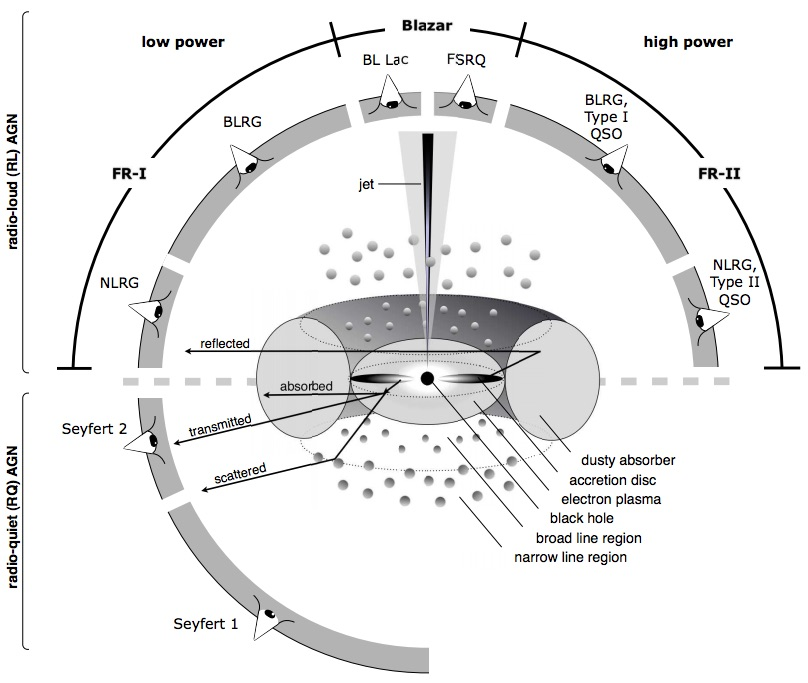
\includegraphics[width=0.849\textwidth]{images/misc/agn_model.jpg}%{}{}
    %}
    \caption{A simplified schema of the current model of the AGN, not drawn to scale. The taxonomy of the AGN is a result of the presence or absence of various components and observational effects. Figure reproduced from \citet{beckmann2012agn}.\label{fig:agn_model} }
\end{figure*}
 Figure \ref{fig:agn_model} shows a simplified view of the default AGN model.  A SMBH at the center forms the \textit{central engine}, accreting matter via an accretion disk. For powerful systems, the spectrum of the disk peaks in the optical/UV and is traditionally called the ``big blue bump." The accretion disk photoionizes the neighboring high density and dust-free gas clouds, which leads to the production of strong  emission lines. These clouds mostly occur within a parsec of the SMBH \citep{peterson2006broad}; they move with roughly keplerian speeds, and, as a result,  broaden the emission lines. Hence, this region is known as the broad-line region (BLR). The low-density, low velocity, ionized gas, residing a few hundred to thousands of parsecs away from the black hole, moves with slower speeds, and produces narrower emission lines. This region constitutes the narrow-line region (NLR). A dusty torus structure may also surround the black hole-disk system. When viewed edge-on, this torus obscures the emission from the BLR. Such sources lack broad emission lines and fall under the Type II class of AGN. If the AGN are observed face-on, the broad emission lines become visible, and are categorized as Type I AGN. This viewing angle based classification plays an important role in understanding the AGN, although it is clear that the torus is likely more complex and ``clumpy" that what is shown here \citep[see][and references there in]{H_nig_2019}.
 \subsection{AGN Taxonomy \label{sec:taxonomy}}
AGN were classified, traditionally, as radio-loud and radio-quiet, in an empirical sense. The dividing factor was the ratio of radio to optical flux density ($R$). Those with $R\leq10$ were classified radio-quiet (but are not radio-silent) and those above the limit radio-loud. However, this classification has been criticized in the recent times for its oversimplification \citep[e.g.,][]{Padovani_2016}. For example, the emission in the optical band may be dominated by the jet itself, and can lead to $R<10$, thereby incorrectly classifying sources as radio-quiet. Hence this distinction is not just taxonomic but an intrinsic one. It stems from the presence or absence of a jet \citep{Padovani_2017}. Hence, in what follows, they would instead be referred to as jetted and non-jetted AGN, respectively.
\subsubsection{Jetted AGN}
\textit{Radio Galaxies} (RG) are the initial detections of jetted AGN with identified optical counterparts \citep[e.g.,][]{1954ApJ...119..215B}. They are AGN with jets that are aligned away from our line of sight. RGs are further classified in to two types based on their optical spectra: broad line (BLRG), which display both broad and narrow emission lines, and narrow line (NLRG), which only display narrow lines  (see Fig~\ref{fig:agn_model}).  \citet{fanaroff1974morphology} found that the morphology of the large-scale jet occured in two main flavours and correlated with its low-frequency radio luminosity. It was later found that the same also exists in the radio-optical luminosity plane \citep{owen1994fri}. The lower power Fanaroff-Riley Class I (FR I) jets display a plumy structure which fade away with distance from the \textit{core}, which forms the base of the jet. The left panel in Fig.~\ref{fig:FR_I_II} shows a radio image of M84, a typical case of FR I jet. In contrast, the more powerful FR-II type jets, which are the main focus of my thesis, remain highly collimated and travel to much longer distances before they ram in to the inter-galactic medium terminating in a bright \textit{hotspot} where the electrons are re-accelerated before escaping into the lobes. It were these gaint radio-emitting lobes that appeared as extended structures in the initial sky surveys. In general, sources with luminosity at 1.4 GHz $L_{1.4GHz}<5\times10^{25}~\textrm{W Hz}^{-1}$~
%[UNITS. ALSO IT IS BEST TO MENTION THE 178 MHZ AT WHICH FR DO THE SEPARATION, AS IT IS LESS CONTAMINATED BY THE BEAMED CORE]
belong to the FR I class while most of those above the limit to the FR II class. Note that, \citet{fanaroff1974morphology}originally divided sources into FR-I and FR-II classes using the luminosity at 178 MHz which is expected to be dominated by isotropic emission from the c
\begin{figure}
        %\gridline{
    %\boxedfig{images/misc/3C272.1_FR_I_example}{0.35\textwidth}{(a) FR I}
    \begin{subfigure}[t]{0.365\textwidth}
        \frame{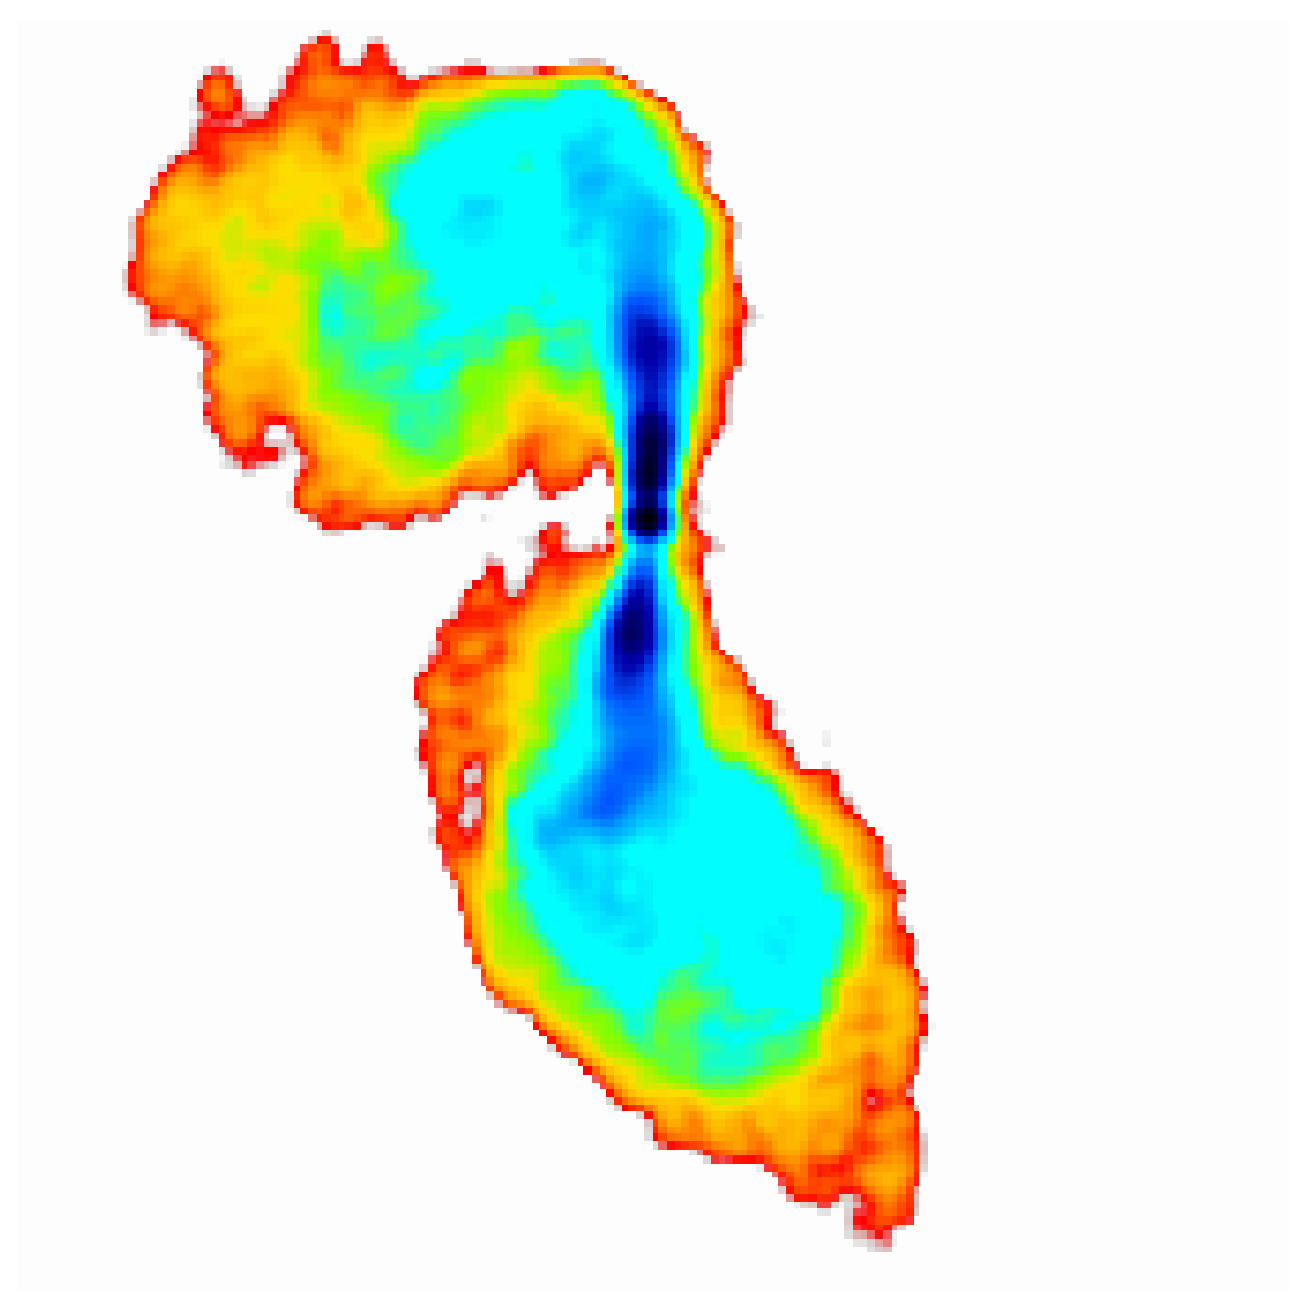
\includegraphics[width=\textwidth]{images/misc/3C272.1_FR_I_example}}
        \caption{ M84, an FR I jet}
    \end{subfigure}
    \begin{subfigure}[t]{0.635\textwidth}
        \frame{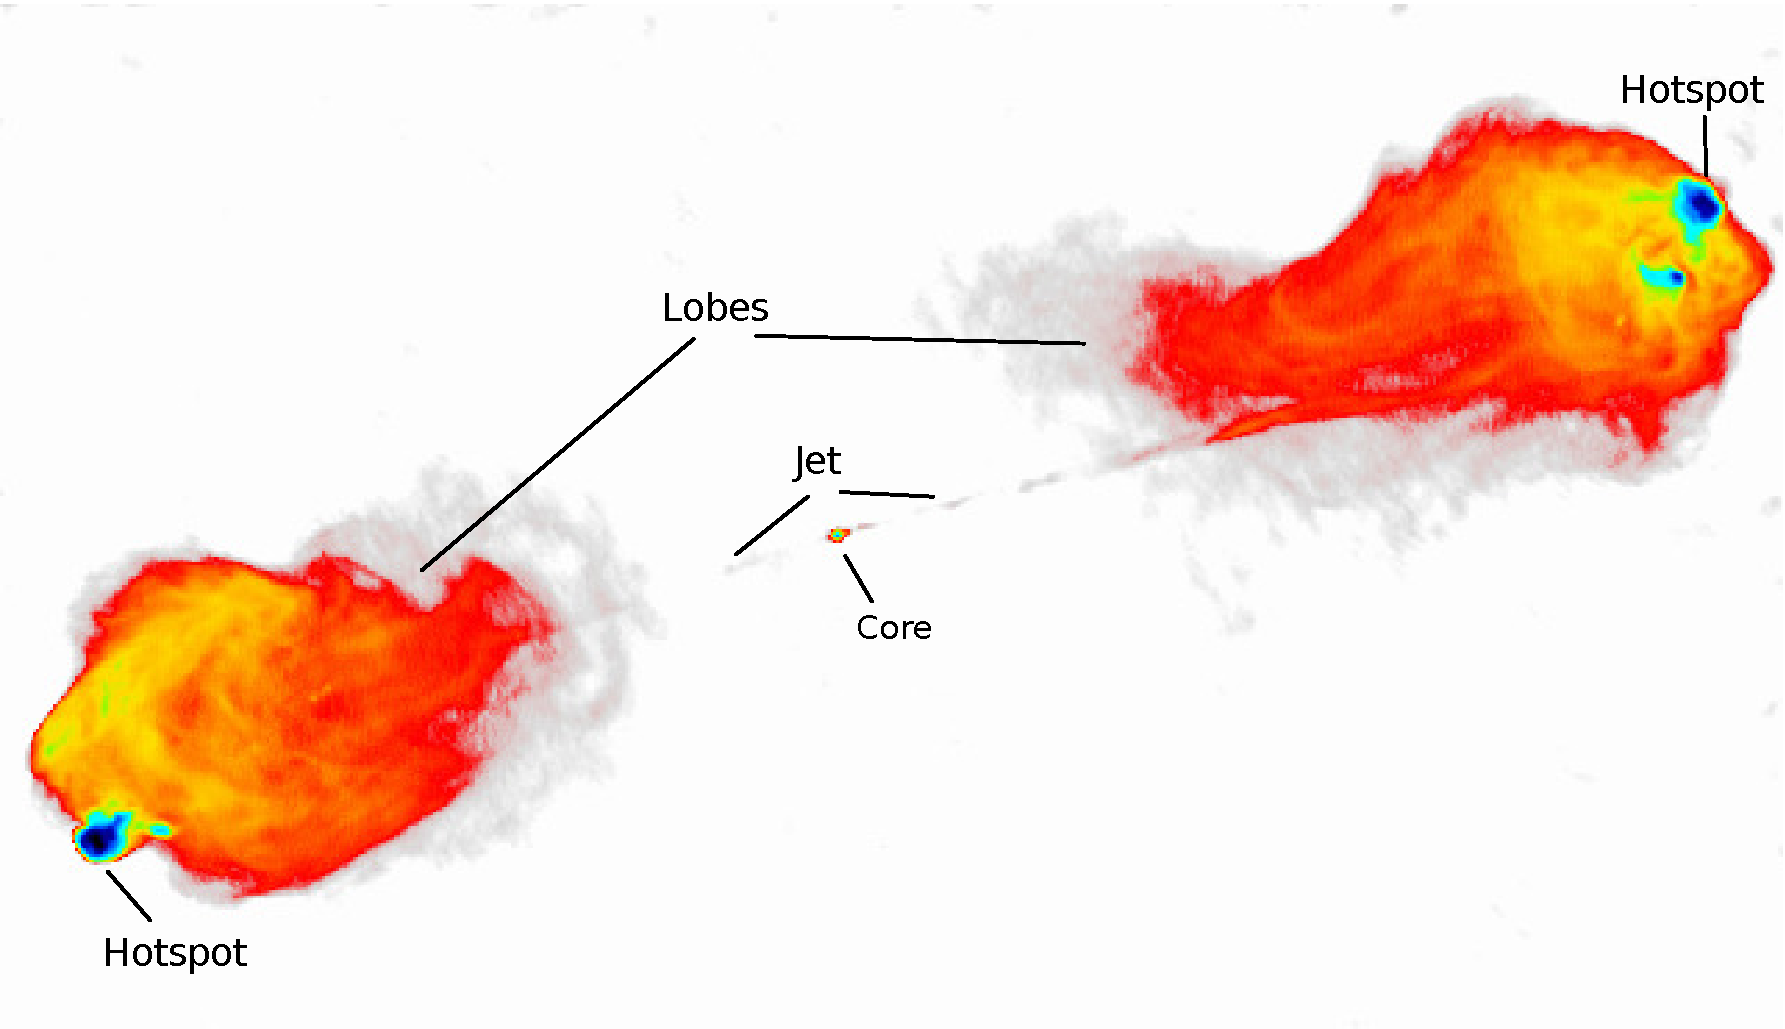
\includegraphics[width=\textwidth]{images/misc/CygA_FR_II_example-eps-converted-to-annotated.pdf}}
        \caption{Cygnus A, an FR II jet}
    \end{subfigure}
    %\frame{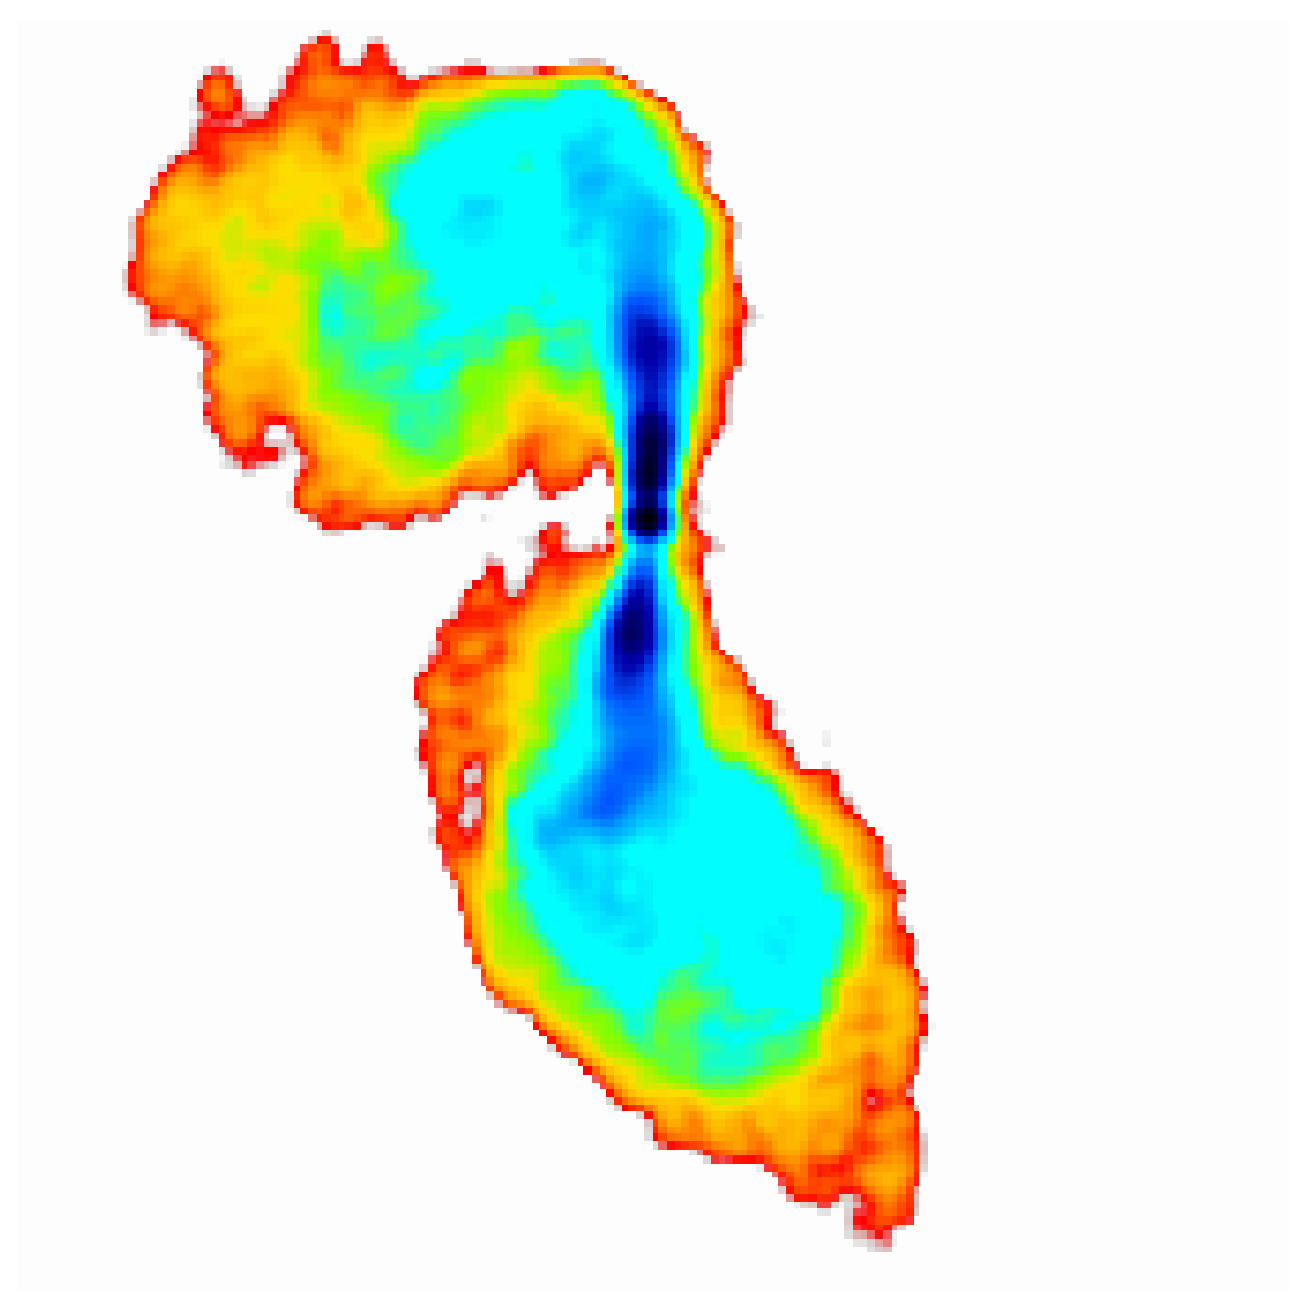
\includegraphics[width=0.365\textwidth]{images/misc/3C272.1_FR_I_example}}
    
    %\boxedfig{}{0.607\textwidth}{(b) FR II}
    %}
    \caption{Typical example images for the FR I and II classes. (a) shows a VLA radio image of an FR-I source, M84, where the where the jet's brightness gradually decreases with increasing distance from the core (image taken from DRAGN website, http://www.jb.man.ac.uk/atlas/). (b) shows a a radio image of an FR-II source, Cygnus A. Two jets originate from the core and terminate in bright hotspots, feeding accelerated plasma into the radio lobes (image taken from NED, http://ned.ipac.caltech.edu).\label{fig:FR_I_II} }
\end{figure}

\textit{Quasars} comprise the most powerful class of jetted-AGN with their jets aligned at relatively smaller angles than FR I/II sources. They are typically characterized by the presence of broad emission lines in the optical spectrum and high luminosity radio emission. Quasars are classified into Steep Radio Spectrum Quasars (SRSQ) and Flat Spectrum Radio Quasars (FSRQ). SRSQs are dominated by emission from their radio lobes, which usually have steep spectra ($\alpha>$0.5). FSRQs,  often referred to as \textit{Blazars}, are dominated by emission from the cores, which usally have flatter spectra ($\alpha<$0.5). Their jets aligned very close to our line of sight, and typically appear point-like in radio maps with their jets barely visible due to extreme foreshortening. They are are further divided into two classes: FSRQ, which display broad emission lines, and BL Lacertae objects (BL Lacs), which have featureless spectra. Under the primary unification scheme 
\citep[e.g.,][]{urry1995unified}, FSRQs and BL Lacs are the closely aligned counterparts of FR II and FR-I RGs, respectively. Blazars have the highest apparent luminosity of all AGN families with Doppler beaming capable of enhancing the intrinsic luminosity by a factor of up to $10^9$. Historically, quasars were also classified into lobe-dominated quasars (LDQ) and core-dominated quasars (CDQ). LDQs (and FR II RGs) are mainly detected in low-frequency radio surveys which are dominated by isotropic emission from lobes. On the other hand, CDQs are mainly detected in high-frequency radio surveys which are dominated by emission from the cores. 

%The sources that are intermediate between radio galaxies and blazars are called Steep Spectrum Radio Quasars (SSRQs). The radio spectrum of the SSRQs is steeper than that of blazars, as there is a contribution from the lobe, which has a steeper spectrum, as opposed to the core, which has a flatter spectrum. Because of a major contribution from the beamed emission from the core, blazars appear as ``core dominated" while emission from the lobes constitute a major contributor to the observed emission in radio Galaxies, and hence they appear as ``lobe-dominated" \citep{1997iagn.book.....P}.
%Typically, the blazar category sources are observed to be ``core dominated"; the bulk of their radio emission comes from the relativistically beamed core. In contrast, the radio galaxies are observed to be ``lobe dominated"; the bulk of their radio emission comes from the lobes, which are not beamed. As the blazar jets are closely aligned, the beamed emission from their core overwhelms the emission from the lobe. Because the jets are aligned away from us in the radio galaxies, the emission from their lobes surpasses the de-beamed emission from their core.



\subsubsection{Non-jetted AGN}
These are the most common class of AGNs in the local universe, and Seyfert galaxies \citep{seyfert1943nuclear} were the first ones to be identified in this class. Seyfert conducted his research using the telescopes at Mt. Wilson, which also hosted prominent researchers indlucing Edward Hubble who pioneered extragalatic studies and Albert Michelson who worked on interfgerometry.

Typically, the Seyferts are distingusihed from other normal galaxies by their highly ionized emission lines and luminous cores. Similar to jetted-AGNs, the Seyfert galaxies are divided into two classes based on their optical spectra \citep{khachikian1974atlas}: Seyfert I type, which display narrow and broad emission lines, and Seyfert II type, which only display narrow emission lines (see Fig.~\ref{fig:agn_model}). Apart from the optical classification, the Sefyferts are also classified based on their X-ray emission, which relies on the intrinsic absorption in the soft X-ray band ($E\ll 5~\textrm{keV}$). A hydrogen absorption column density of $N_H=10^{22}~\textrm{cm}^{-2}$ draws the line between the type I and type II Seyferts. The ones above the threshold are strongly absorbed and fall into the type I class, while the ones below have lower absorption and fall into the type II class.  Radio-quiet quasars are another type of non-jetted AGN. Similar to the Seyferts, the radio-quiet quasars are further divided in to type I and type II, which display broad lines and only narrow lines, respectively.
                                                               
There may also be sources with a low luminosity that go undetected in the all-sky surveys. For example, the bolometric luminosity of Sagittarius A*, which is the black hole at the center of our Milky Way galaxy, is less than $L_{bol}=10^{37}~\textrm{erg sec}^{-1}$. Such emission would not be detected if it were to lie in a distant galaxy. It is believed that these sources may have experienced some activity in the past and are presently undergoing a quiescent phase.

\subsection{The Central Engine \label{sec:engine}}
The idea of a black hole at the center of AGN was a groundbreaking one as it explained puzzling features of the AGN such as short variability time scales and extremely high luminosity \citep{salpeter1964accretion,zel1964estimating,lynden1969galactic}. It is now widely believed that accretion on to an SMBH power all forms of AGN. 

%and it could not be due to a single massive star. Their short variability time scales imply a tiny emitting region as any significant change in the luminosity can only occur on times greater than the light-crossing of the emitting region. This led to the idea that accretion on to SMBH powers the radiative output of quasars , which is the currently accepted model.

\subsubsection{Detecting SMBH in AGN}
Although the idea of an SMBH at the center of an AGN was rapidly adopted by the community, it took a long time to infer the presence of black holes. So indirect methods that revealed the gravitational influence of black holes on their surroundings became the key. For example, star trajectories around the presumed location of a black hole can be monitored to infer its presence. However, they typically orbit around SMBHs on sub-parsec scales. Hence, this method could only be applied to a few nearby galaxies that allowed telescopes like HST to track proper motions of individual stars. Indeed, the properties of the SMBH at our galaxy's center remain the most precise ever to be measured using this method \citep{2008ApJ...689.1044G}.

Reverberation mapping is another important technique that was developed in the 1990s (see \citet{Peterson2004} for a review) to measure the properties of SMBHs. In the default picture of AGN, the continuum from the accretion disk ionizes the gas clouds in the BLR that, in turn, emit emission lines. Broader line-widths are expected from regions closer to the black hole because of faster speeds and stronger gravitational fields. Hence, any change in brightness of the continumm must also lead to a change in the brightness of the emission lines but with an associated time lag. Because any correlated events can only happen on timescales greater than the light-crossing time between two regions, these time lags place can be used to place an upper limit on the size of the BLR and also determine the mass of the black hole \citep{Peterson2004}. 

Another key insight was gained in the 1990s, where it was found that the mass of a galaxy's SMBH correlates with the surrounding spheroidal distribution of stars known as the galactic bulge \citep{magorrian1998demography}. The observed stellar velocity dispersion at the center of a galaxy is known to scale with its bulge mass. This dispersion is currently used to estimate the mass of the SMBHs and is known as the $M-\sigma$~relation
\citep{ferrarese2000fundamental,gebhardt2000relationship}. Recently the Event Horizon Telescope provided a direct evidence of SMBH by imaging the central region of M87 \citep{2019ApJ...875L...1E}.
%[CITATION]
\subsubsection{Disk Accretion and the Eddington Limit\label{subsec:accretion}}
The accretion process is extremely efficient at converting the gravitational potential energy of infalling matter into radiation. ``Spherical" type of accretion, commonly called \textit{Bondi} accretion \citep{bondi1952spherically},  that was was the first type to be sturied. Bondi accretion is only a good approximation for isolated compact objects and is unlikely to be the main process behind AGN activity. It is because of the lack of angular momentum in spherical accretion: the particles do not have time to radiate their thermal energy before they fall in to the black hole. However, if the in-falling matter forms a disk while possessing angular momentum, its radiative efficiency can be significantly higher. In the case of objects like AGN, an accretion disk will be formed.  The bolometric luminosity of the accretion disk is given by $L_{acc}=\eta\dot{M}c^2$, where $\dot{M}$ is the accretion rate and $\eta$~is the radiative efficiency of the disk. The efficiency parameter $\eta$ can range between 0.06 and 0.3 and is determined by several parameters including spin of the black hole, the type of accretion that are far from a clear understanding \citep{raimundo2009eddington}.
%[NEWER CITATION]  

In 1920s, Arthur Eddington noted that for a spherical mode of accretion, the radiation from the inner parts of the in-falling matter would exert pressure on the outer parts, thereby limiting the maximum achievable luminosity. The limiting luminosity depends on the type of the in-falling matter, which is generally taken to be ionized hydrogen in most astrophysical environments, and the mass of the black hole. It is called the \textit{Eddington} luminosity. For a black hole that predominantly accretes ionized hydrogen, the Eddington luminosity (in ergs s$^{-1}$) is given by
\begin{equation}
    L_{edd}\simeq1.3\times10^{38}\frac{M}{M_\odot}{\rm erg/
    s} 
    \simeq 3\times10^4\frac{M}{M_\odot}L_\odot
\end{equation}
where $L_\odot$ is the solar luminosity. A bright quasar typically has a luminosity of $\sim10^{13}L_\odot$, which then implies a black hole mass of  $\geq3\times10^8M_\odot$, indicating the super massive nature of black holes powering AGN. Note that $L_{edd}$ is derived assuming spherical accretion and may be inaccurate for real systems where matter orbiting around SMBHs is expected to for a disk. Multiple other processes can also influence the $L_{edd}$. For example, highly-ionized heavier elements in the infalling matter can decrease the luminosity by absorbing spectral lines. Conversely, low-ionized counterparts practically remain transparent to the outgoing radiation, increasing the luminosity. Furthermore, any anisotropy in the distribution of the in-falling matter will accordingly decrease $L_{edd}$ \citep{frank2002accretion}. These limiting factors clearly indicate $L_{edd}$ only provides an order of magnitude estimate for the limiting luminosity, and accreting rate may exceed this value as observed in multiple AGN \citep[e.g.,][]{2014ApJ...793..108W,liu2021observational} . 
%[NOT CLEAR].
%Although, in principle, Bondi accretion may take place in nearby non-active galaxies, the observed X-ray flux is orders of magnitudes smaller than what is expected \citep[e.g.,][]{wong2011resolving}, indicating the presence of an even more inefficient accretion process.
%[WHO CLAIMS THAT?]
\subsubsection{Jet launching}
The precise means by which the jets are accelerated by SMBHs remain unclearn as is the matter content of the jet plasma. Over the years, many published jet launching mechanisms have commonly assumed that the jets acquire their mass from a certain fraction of the accreting matter. However, they differ in whether or not the magnetic field is primarily responsible for ejecting the jet.

Pure hydrodynamic models based on winds from accretion disks such as those powered by binary black holes \citep[e.g.,][]{1973A&A....24..337S} have limited capabilities. They cannot accelerate the jets to relativistic speeds, generally seen in VLBI observations. In contrast, low-efficiency accretion flows may produce adequately relativistic outflows with reasonable collimation \citep{rees1982ion,das1998observational}. However, these models rely on some critical assumptions that are yet to be verified.

The current belief is that magnetic fields play an important role in launching the jet and collimating them. One observational aspect supporting this view is radio emission from jets, which, by definition, requires a magnetic field. Also, magnetic fields can naturally produce relativistic speeds and collimated outflows with large kinetic energies \citep[e.g.,][]{heinz2000jet}, making magnetic field models superior to pure hydrodynamic models. 

The magnetic field models generally come in two flavors. They either harvest energy and angular momentum from the accretion disk \citep[e.g.,][BP]{blandford1982hydromagnetic}, or from the spin of the black hole that threads the magnetic field at its horizon \citep[e.g.,][BZ]{blandford1977electromagnetic}. For the BP mechanism, one would expect a tight correlation between the accretion power and jet power, which is observed in some Galactic systems \citep[e.g.,][]{willott1999emission}. However, there is also evidence for correlation between black hole-spin and  jet power \citep[e.g.,][]{mcclintock2013black} with recent 3D relativistic magnetohydrodynamic simulations of jets supporting this scenario \citep{mckinney2006general,tchekhovskoy2011efficient,marti2019numerical}.
%Nevertheless, gaining deep insights into the physics of the jet launching would likely require more detailed large scale numerical simulations. 

%It is important to note that most of the simulations reproduce the observed properties of jets. However, they might not represent the actual conditions that exist in a jet. [NOT REALLY TRUE. MOST SIMS DO NOT HAVE PARTICLE ACCELERTION COUPLED TO MHD AND THEY DO NOT HAVE PROPER RADIATIVE PROCESSES AND COUPLING TO THE JET FLOW]

Another important unknown is the particle composition of the jet. The material that transports energy and momentum from the parsec scales of the AGN out to kpc and Mpc scales is still uncertain. As mentioned, this material may not necessarily be the radiation-emitting plasma. For example, electrons with energies $\gamma\geq2000$\footnote{$gamma=\frac{1}{\sqrt(1-(v/c)^2} $is the Lorentz factor} would not survive until the tip of the jet  \citep{2007RMxAC..27..188H} and hence cannot be the energy carriers of a jet. A few possibilities for the jet material include cold (thermal) or hot (relativistic) protons, cold electrons/positrons, or Poynting flux (energy stored in magnetic fields).  Although neutrons were also suggested as a candidate jet material \citep{dermer2004nonthermal} it faced difficulties with jet formation and jet bending on kpc scales. \citet{sikora2000pair} argued that protons are the main energy carriers of the jet but electrons (and positrons) outnumber them. \citep{sikora2005quasar} extended this argument by suggesting that the Poynting flux dominates the jet initially and the particles would dominate later with protons mainly carrying the energy of the jet. Hoever, observations of FR II radio-lobes indicated that those jets are more likely to be dominated by pair plasma.

The location where the jet reaches its peak Lorentz factor is also uncertain. It could happen extremely close to the black hole, or the jet could be progressively accelerated while propagating away from the black hole  \citep[see~][]{meier2003theory}. The latter mode is commonly adopted because if the jet is accelerated close to the black hole, it will experience significant energy loss by inverse-Compton scattering (see section \ref{subsec:ic}) of the ambient photon field, a phenomenon that is commonly known as the ``Compton drag" effect.
More detailed observations, theoretical studies, and numerical simulations are necessary to resolve these questions.

\section{X-ray jets\label{sec:xray_jets}}
``A curious straight ray lies in a gap in the nebulosity in p.a. $20^\circ$, apparently connected with the nucleus by a thin line of matter. The ray is brightest at its inner end which is 11\as~from the nucleus", \citet{curtis1918descriptions} noted, while describing the optical image of an elliptical galaxy, \textit{NGC 4486}. This is considered as the first-ever detection of an astrophysical jet which we now recognize as the jet from M87. While radio and optical telescopes detected several jets by 1990s, it took a few more years for them to be properly resolved in the X-rays.

The construction of X-rays observatories based on gas proportional counters began in the 1950s, and were able to X-ray emission from AGN around early 1960s and late 1970s.  However, they could not resolve jets due to low angular resolution. Later, the \textit{Einstein} X-ray observatory was launched in 1978; it had a resolution of $\approx$5\as~and was able to resolve nearby jets from the core in nearby sources M87 \citep[][]{schreier1982high}. The launch of \textit{ROSAT} soon followed in 1990, which had similar capabilities but with higher sensitivity. It was able to detect other nearby jets, including, the hotspots from Cygnus A and 3C 390.3 \citep{reynolds1996rosat,almudena1997extended}. Nevertheless, the poor angular resolution of both  observatories precluded the detection of jets from distant sources as they required sub-arcsecond resolution.

\subsection{The Chandra X-ray Observatory}
The dection of distant X-ray jets was made possible by \textit{Chandra}, an X-ray observatory with an unprecendented angular resolution of \siml0.5\as. \textit{Chandra} observes the sky between the energy range of 0.2-10 keV and remains one of the biggest drivers for jet physics studies in the recent times. After \textit{Chandra} was injected into the orbit, the ground team selected a distant quasar, PKS 0637-752, with a 100 kpc long radio jet, to calibrate the telescope. Because PKS 0637-752 was expected to be a bright point source in the X-rays, it was also going to serve as a calibrator for the telescope's in-focus measurements. However, with only a 2 ks exposure on this source, a faint bridge-like structure appeared to the west of its core, along the same position angle as the radio jet. This detection marked \textit{Chandra's} first serendipitous discovery of an X-ray jet \citep{chartas2000chandra}. The left panel of Figure \ref{fig:pks0637-752_show_piece} shows a 100ks \textit{Chandra} image of this source, while the right panel shows its 8.6 GHz radio image.

%Presently, more than 150 of the radio jets stand detected in the X-rays by \textit{Chandra} \citep[e.g.,][]{sambruna2004survey,marshall2005chandra,massaro2015chandra}.
\begin{figure*}
    \gridline{
    \boxedfig{images/misc/pks0637_initial_xray_image}{0.42\textwidth}{(a) \textit{Chandra} X-ray image}
    \boxedfig{images/misc/pks0637-752_intial_radio_image.png}{0.42\textwidth}{(b) ATCA 8.6GHz radio image}
    }
    \caption{The X-ray and radio images of PKS0637-752, the first detection of an X-ray jet by \textit{Chandra}. Image taken from \citet{chartas2000chandra}    \label{fig:pks0637-752_show_piece} }
\end{figure*}
%The X-ray jet is about \siml100kpc and closely follows the radio until a bend in the jet. This suggested that the X-ray jet may be more beamed away from us than the radio. But there is only a weak detection of  optical emission from the knots. 
 The radio-to-X-ray spectrum of FR-I jets is generally consistent with a single synchrotron component \citep[e.g.,][]{Marshall_2002,Hardcastle_2003} suggesting that a single electron population with a powerlaw distribution of energies produce the emission via synchrotron mechanism \citep[for a notable exeception, see][]{meyer2018detection}.  However, nearly in all the sources with an FR II-type jet like PKS 0637-752, the observed X-ray emission is a few orders of magnitude brighter than an extension to the radio and optical (if present) spectrum \citep[e.g.,][]{sambruna2004survey,marshall2005chandra,2011ApJ...730...92H,2011ApJS..193...15M,marshall2018x}, clearly requiring a second spectral component. Following \citep{breiding2017fermi}, I refer to these jets as ``Multi Spectral component (MSC)'' jets. The left panel of Figure \ref{fig:w7.8_sed} shows the observed spectrum of a discrete feature or a ``knot'', W7.8, in PKS 0637-752 as an example. The solid line indicates the low energy synchrotron spectrum with no detectable level of X-ray flux. Moreover, invoking thermal processes for the genesis of X-rays in this jet implied unrealistic electron densities and higher than observed rotation measures \citep{schwartz2000chandra}. While SSC flux under equipartition fell short of the observed X-ray flux at least by a factor of 100, IC scattering the cosmic microwave background CMB (IC/CMB) by a non-relativistic jet underpredicted it by about three orders of magnitude \citep{chartas2000chandra}. 
 
 %The individual detection papers of PKS 0637-752, \citep{schwartz2000chandra,chartas2000chandra} report that the usual mechanisms to explain the observed X-ray emission do not work. Thermal emission would produce larger than observed rotation measure and implies an implausible electron density. The synchrotron-self Compton (SSC) flux falls short of the observed X-ray flux at least by a factor of 100 assuming equipartition. In addition, 
 %[I PREFER NOT TO START A SENTENCE WITH AND OR BUT] 
 %for a non-relativistic jet, the flux produced by relativistic electrons that inverse-Compton scatter the cosmic microwave background (CMB) would under predict the X-ray flux by orders of magnitude. The left panel of Fig.~\ref{fig:w7.8_sed} shows the spectrum of knot W7.8 in PKS 0637-752 which depicts the anomalous nature of the X-ray emission from TSC jets.
\begin{figure}[h!]
    \gridline{
    \boxedfig{images/misc/chartas_w7.8.png}{0.42\textwidth}{(a)}
    \boxedfig{images/misc/tavecchio_2000_sed.png}{0.42\textwidth}{(b)}
    }
    \caption{ (a) The spectrum of knot W7.8 of PKS0637-752 where the solid line is the synchrotron component. Under equipartition condition, the dashed line indicates the SSC component while the dotted line, the inverse-Compton component from a non-relativistic jet, and both the mechanisms fail to account for the observed X-ray emission. Image taken from \citet{chartas2000chandra} (b) The Spectral energy distribution (SED) of knot W7.8 of PKS 0637-752. The X-ray emission can be explained by IC/CMB if the jet is closely aligned and highly relativistic, and the up-scattering electrons have low energies (much lower than what is traced by the radio-optical spectrum). Image taken from \citet{tavecchio2000x}.
    %[EXPLAIN THE SECOND ONE BETTER]    
    \label{fig:w7.8_sed} }
\end{figure}

%\textcolor{blue}{What were proposed to solve this problem. Introduce the one zone models.}
\subsection{The IC/CMB model}
A few months after \textit{Chandra} detected its first jet, two independent groups reproduced the X-rays in PKS 0637-752 with IC/CMB  by requiring its jet to be highly relativistic and closely aligned to our line of sight \citep{tavecchio2000x,celotti2001large}. The right panel of Fig.~\ref{fig:w7.8_sed} shows the SED of the W7.8 knot in PKS 0637-752 with an IC/CMB component consistent with the obsereved X-ray flux. Until recently, the IC/CMB model remained the leading explanation for X-ray emission from MSC jets \citep[e.g.,][]{sambruna2004survey,miller2006x,sambruna2006jet,2012ApJ...748...81K}. However,
it failed to describe multiple spectral and structural characteristics of MSC jets.
%A similar model involved the idea that the jet can also upscatter photons from the central nucleus to produce \citep[e.g.,][]{2001MNRAS.321L...1C}. 
%($\gamma_{min}\sim 30-100$) with energies much smaller than those tracing the observed GHz spectrum ($\gamma\sim10^4$)
%the X-ray emission from the lobes of  the IC/CMB model has been the leading
\subsection{Issues with the IC/CMB model}
Under equipartition conditions, electrons tracing the GHz spectrum typically have $\gamma\sim10^4$, much larger than the  energies required by IC/CMB ($\gamma\sim 30-100$) to produce X-rays. Extending the electron energy distribution (EED) to low energies requires introducing a significantly larger number of electrons into the jet and may make its kinetic power to exceed the Eddington luminosity  \citep{dermer2004nonthermal}. Moreover, the EEDs need an \textit{ad-hoc} cutoff at low energies (e.g., $\gamma_{min}=10$) to prevent overproducing the optical emission. Even if the IC/CMB electrons exist in jets, their synchrotron emission possibly lies below the ionospheric cutoff making it impossible to detect them with the modern day telescopes. In contrast, low-frequency radio maps of the lobes of radio galaxies, which are non-relativistic and emit isotropically with $\gamma\sim10^3$, provide direct evidence for IC/CMB mode of X-ray emission   \citep[e.g., ][]{1995ApJ...449L.149F}.

Beside low-energy electons, the radio-optical emitting electrons will also up-scatter the CMB photons to produce  GeV emission. Its flux-level is predetermined by the requirement of reproducing the X-ray emission \citep{georganopoulos2006quasar}. Properly, the SED of the IC component is a scaled and translated version of its low-energy counterpart. However, upper limits on GeV emission from the jets in many quasars, including PKS 0637-752, obtained by the \textit{Fermi} imply much lower values than the predicted level \citep{meyer2015ruling,breiding2017fermi}. 

Since the radio and X-rays are produced by the same electrons, their spectral indices are expected to match. While low-count statistics of the X-ray spectra prevent an accurate comparison between X-ray and radio spectral indices for many jets, high-sensitivity \textit{Chandra} observations of a well studied nearby jet,  3C 273, indicate a clear disagreement between X-ray/radio spectral indices \citep{jester2006new}.

%A single synchrotron component describes the radio to IR spectra from its resolved knots \citep{uchiyama2007infrared}. On the other hand, i
Another argument against IC/CMB comes from UV polarimetry of
PKS 1136-135, a unique source where, unlike in most of the MSC jets, the UV emission lies on the low-energy tail of the second spectal component. For IC/CMB to produce the observed UV to X-ray spectrum, the upscattering electrons must have $\gamma\sim$ few for the UV and $\gamma\sim100$ for the X-rays \citep{uchiyama2007infrared}. Because the CMB is unpolarized, X-rays are expected to be unpolarized UV emission to be slightly (few percent) polarized  \citep{uchiyama_2008,mcnamara2009x}. However, the fractional polarization in the UV exceeds \siml30\% in several knots, ruling out IC/CMB \citep{cara2013polarimetry}.
%\textcolor{blue}{Offsets}

The knotty morphology observed in several X-ray jets presents a problem for the IC/CMB model \citep[e.g.,][]{sambruna2004survey,jester2006new,Clautice:2016zai,siemiginowska2007300}. While the mechanism producing knots is unknown, the large radiative cooling times of the X-ray emitting electrons  \citep[$\geq 10^6$ years, e.g.,][]{harris2006x} implies no significant X-ray brightness variations must be observed along the jet as opposed to the observed knots with differing brightnesses. Although separate moving blobs of plasma with large bulk Lorentz factors ($\Gamma>10$) can still produce X-rays knots emitting via IC/CMB \citep{tavecchio2003clumps}, optical proper motions in the knots of nearby jets indicate much smaller values \citep[$\Gamma<2.9$ in 3C 273, e.g., ][]{meyer2016hst}. Moreover, assuming moving knots are made of several smaller clumps can  explain X-ray flux variations in knots via adiabatic losses. However, these losses may produce a large poulation of electrons capable of overproducing the optical emission via IC/CMB \citep{stawarz2004multiwavelength}.

Long cooling times also imply multiple other properties. First, no variability in the X-ray flux would be expected on human time scales unlike a knot in Pictor A that varied significantly in a few years \citep{marshall2010flare}. Second, because of the relatively smaller lifetimes of GHz radio-emitting electrons, as noted by \citet{worrall2009x}, we should expect the X-rays to extend beyond the radio or at least be co-spatial, appearing as if being emitted from a ``single zone'' in the jet. However, the X-rays peak and decay before the radio in many knots of MSC jets \citep[e.g.,][]{2005MNRAS.360..926W,siemiginowska2007300,kataoka2008chandra,worrall2009x,Clautice:2016zai}, generally manifesting as peak-to-peak positional \textit{offsets} between X-rays and radio. Figure \ref{fig:3C111} shows the X-ray image of 3C 111, overlaid with 8.4 GHz radio contours. Offsets can be seen, for example, in knots K9, K30, K45. Although we are far from understanding how offsets are produced, they place an important constraint on the emission morphology and, in turn, the X-ray emission mechanism: the bulk of the X-ray and radio emissions are produced in different zones of the jet, contrary to IC/CMB's single zone operation. It is important to note that this constraint applies independent of the emission mechanism.

\begin{figure}
    \centering
    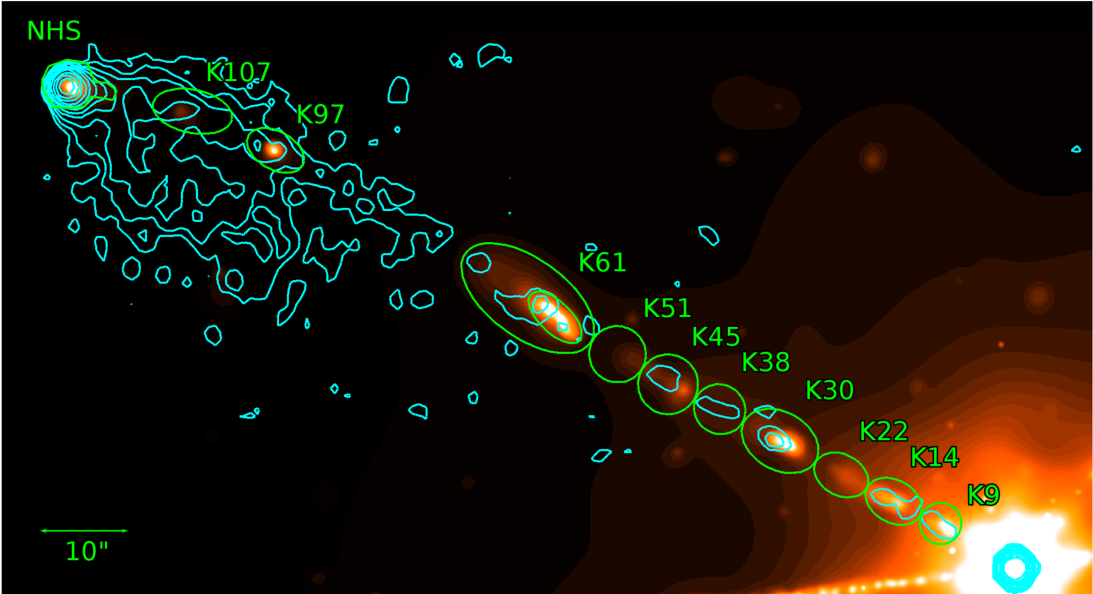
\includegraphics[width=0.8\textwidth]{images/sources/3c111.png}
    \caption{A smoothed X-ray image of 3C111, overlaid with the VLA 8.4 GHz radio contours. The X-rays peak and decay before the radio in multiple knots including K9, K30, K45, K61, which appear as peak to peak offsets. Image taken from \citet{Clautice:2016zai}}
    \label{fig:3C111}
\end{figure}

\subsection{Modified IC/CMB and Alternatives}
A major issue with the IC/CMB model from the beginning was its requirement for the jet to remain relativictic  ($\Gamma\sim10$) even on kpc scales. In contrast, all radio-based studies on large scale jets implied that radio jets only mildly relativistic~\citep[$\Gamma\lesssim 1.5$, e.g., ][]{wardle1997fast,mullin2009bayesian}. One clue came from the observations of X-ray fluxes that decreased with distance from the core. \citet{hardcastle2006testing} noted that although IC/CMB coupled with jet deceleration can explain this decline, the cold matter required to entrain the jet in many cases is implausibly high. The author suggested that a transverse velocity structure (e.g., a fast X-ray spine enclosed by a slow radio sheath) must exist in MSC jets for IC/CMB to be still viable. Stratified velocity structures are not new and are established in many FR I jets \citep[e.g.,][]{laing2004adiabatic,canvin2004relativistic}. While a spine-sheath structure is detected in the parsec scale jets of MSC jets \citep[e.g.,][]{2021A&A...654A..27B}, its presence is yet to be confirmed on kpc scales.

One of the first invocations of spine-sheath models for MSC jets was made in the case of 3C 273. Although it satisfactority reproduced the observed X-ray fluxes from knots, it required unrealistic bulk Lorentz factors ($\Gamma\sim $50-100) for the spine. Moreover, as mentioned, it could not explain the disagreement between X-ray radio spectral indices. \citet{siemiginowska2007300} considered a variant for the case of PKS 1127-145 with a ``proper'' jet consisting of a regular spine and sheath, and a ``sheath'' representing an extension to the jet's boundary layer. Although this model explained multiple aspects of the broadband emission from the knots in PKS 1127-145, it sometimes required extreme changes in the magnetic fields between knots. Nevertheless, the evaluated two-zone IC/CMB models lack a natural explanation for the observed offsets.

Motivated by the problems with IC/CMB model, several workers in the field sided with an alternative, the synchrotron mechansim \citep[e.g.,][]{jester2006new,hardcastle2006testing,Clautice:2016zai}. Producing X-ray via synchrotron would require a high-energy electron population with energies that extend up to 100 TeV (much lager than $\sim1$~TeV electrons that produce radio/optical emission). While this explanation relaxes many constraints imposed by the IC/CMB model, for example, close alignments or large bulk Lorentz factors, it also requires cutoff at a few TeV to avoid overproducing optical emission. Moreover, as noted by \citep{schwartz2000chandra}, introducing a second synchrotron population is ad-hoc in nature  \citep{schwartz2000chandra}--we have no explanation for its existence. \citet{dermer2002x} suggested that a single electron population producing radio-to-X-ray emission via synchrotron emission can devlop a harder tail at X-ray wavelengths owing to inefficient IC losses in the Klein-Nishina regime, resulting in a two component SED. This model requires the radiative losses be more pronounced in IC compared to synchrotron.  Hadronic models may also produce X-rays via synchtrotron, eliminating the need to introduce a second population of electrons \citep[e.g.,][]{aharonian2002proton,petropoulou2017tev}. However, these models require a large proportion of protons, which in turn implies large jet powers,  and magnetic fields on the orders of several Gauss, which are difficult to produce hundreds of kpcs away from the central engine.

The cooling times of X-ray emitting synchrotron electrons are on the order of a few years \citep{harris2006x}. That means, presence of X-ray knots on hundreds of kpc away from the central engine requires \textit{in-situ} acceleration of the electrons. Internal shocks \citep[e.g.,][]{stawarz2004multiwavelength,kataoka2008chandra}  or acceleration in a shear turbulent layer \citep[e.g.,][]{ostrowski2002radiation}, for instance, can re-accelerate electrons, but the exact mechanism is not quite clear.

%Offsets also exist in FR-I sources such as \textit{M87} and \textit{3C 66B} \citep{hardcastle2001chandra,Marshall_2002}, which may be explained by synchrotron time lags associated with downstream advection and radiative cooling \citep{bai2003radio}.

\subsection{Knot and Offset Formation}
Besides the uncertain X-ray emission mechanism, the lack of knowledge on how knots form introduces additonal uncertainty in modeling X-rays from MSC jets. For example, as mentioned, it is unclear whether X-ray and radio knots share the same bulk Lorentz factors. Furthermore, the applicability of equipartition conditions to knots is uncertain. It is reasonable to assume that radio lobes, which remain unperturbed for most of its extent, converge towards equipartition. However, knots, which can represent sites of freshly accelerated/accelerating plasma or parts of the jet perturbed by unknown means, may experience enhanced particle or magnetic field densities and may be far from eqipartition.

One possibility is that knots represent stationary re-confinement shocks driven by external pressure gradients\citep[e.g.,][]{komissarov1998large}, which, although, lacks a way to explain offsets. Alternatively, knots could be separate faster moving blobs of the plasma, produced by modulated activity in the central engine  \citep[e.g.,][]{bridle1986collimation,bridle1989unusual,clarke1992origin,stawarz2004multiwavelength}. A forward-reverse shock may then develop at the downstream tip of the blob, producing X-ray (synchrotron or IC/CMB) and radio emission \citep{stawarz2004multiwavelength}. The observed similarities in the knot sizes across multiple radio frequencies and roughly periodically spaced knots in several jets support this model. \citep{kataoka2008chandra} noted in a detailed study of a nearby jet, 3C 353, it is unclear why/how the two shocks produce seemingly different electron populations. They suggested the knots are instead heavy and slow moving blobs of plasma (still produced by modulated jet activity), embedded in a faster and lighter outerflow. A reverse shock can develop at the upstream end of the blob where it interacts with the outerflow, producing X-rays, while the blob coincides with the radio knot. However, this implies a volume-like emission geometry for radio contrary to surface-like indicated by several radio observations \cite[e.g.,][]{swain1998internal}  

While the IC/CMB models lack any offset producing mechanism, the synchrotron models can, in princple, accommodate offsets at the price of manually moving the X-ray emission zone away from its radio counterpart. In addition to the slow moving knot model introduced by \citet{kataoka2008chandra}, offsets can be produced at bends in the jet where an intial strong shock produces X-rays, while a much weaker shock downstream of the jet produces radio \citep{2005MNRAS.360..926W}. Alternatively, offsets may result when accelerated plasma, initially emitting X-rays, emits gradually at longer wavelengths due to synchrotron loses while advecting downstream. This model implies offsets of about 100 kpc, much larger than the observed offsets of a few kpc \citep[e.g.,][]{siemiginowska2007300,Clautice:2016zai}. Although they can be reduced by introducing additonal adiabatic losses due to a laterally expanding jet, the required expansion rates are much larger than what is observed \citep[e.g.,][]{swain1998internal,kataoka2008chandra}.

The multi-TeV electrons in the synchrotron model will inevitably upcatter CMB photons to produce TeV radiation. These TeV photons can heat the intergalactic medium via plasma instabilities \citep[e.g.,][]{broderick2012cosmological,chang2012cosmological} that can suppress the late-formation of dwarf galaxies \citep{pfrommer2012cosmological}. They can also produce the intergalactic magnetic field and the extra galactic gamma ray background \citep{broderick2012cosmological,blandford2019relativistic}. Hence, if the synchrotron model is applicable to MSC jets, it may be an important clue to understand the structure formation in the universe. While the IC/CMB model is not ruled out completely for all jets, it is unclear whether a pure synchrotron can be preferrerd over it. Moreover, uncertainty in the knot formation mechanism makes the situation even more unclear. Nonetheless, if the single-zone IC/CMB model is correct, it would imply significantly larger jet powers and enormous differences in the environmental impact of jets compared to synchrotron-flavored jets.

\section{This Thesis}
Our understanding of the cosmos emerged from simple speculations about gas clouds in the sky to complex processes around black holes driving relativistic jets to millions of parsecs. Although the last few decades have witnessed substantial theoretical and numerical advances in jet physics, several questions such as how SMBHs accrete matter and launch jets, how they remain collimated, how the AGN activity is modulated, what the jets are composed of, how large scale jets produce X-rays, still remain open. 

In the work presented here, in addition to spectral information, I characterize and use offsets of knots in a large sample of MSC jets to constrain their X-ray emission and knot formation mechanisms. In Chapter 2, largely drawn from \citet{2021ApJS..253...37R}, I describe a novel application of a statistical tool to detect offsets in low-count X-ray observations, where Poisson fluctuations and emission from nearby point sources previously precluded such an analysis. In Chapter 3, I extend this approach to a much larger sample of high-count X-ray jets to study trends in offsets and spectral data. This chapter is drawn from a forthcoming publication Reddy et al. (2022) and forms the heart of my theis. In Chapter 4, I will summarize the results of my thesis and describe possible future directions.












